% Intended LaTeX compiler: pdflatex
\documentclass[11pt]{article}
\usepackage[utf8]{inputenc}
\usepackage[T1]{fontenc}
\usepackage{graphicx}
\usepackage{longtable}
\usepackage{wrapfig}
\usepackage{rotating}
\usepackage[normalem]{ulem}
\usepackage{amsmath}
\usepackage{amssymb}
\usepackage{capt-of}
\usepackage{hyperref}
\usepackage{svg}
\author{Zaz Brown}
\date{\today}
\title{BeRGeR\\\medskip
\large Using Braids for Byzantine-Resistant Geometric Routing on Polyhedral Networks}
\hypersetup{
 pdfauthor={Zaz Brown},
 pdftitle={BeRGeR},
 pdfkeywords={},
 pdfsubject={},
 pdfcreator={Emacs 28.3 (Org mode 9.7)}, 
 pdflang={English}}
\usepackage{biblatex}
\addbibresource{../../../../cite/cs.bib}
\begin{document}

\maketitle
\setcounter{tocdepth}{1}
\tableofcontents

\section*{Problem Definition}
\label{sec:orgd417a7b}

\begin{center}
\begin{tabular}{ll}
\hline
\textbf{Online routing} & Nodes are \textbf{myopic} (only see immediate neighbors)\\[0pt]
\hline
\end{tabular}
\end{center}

Robust routing on low-resource devices

\begin{itemize}
\item IoT
\item Sensor networks
\item Vehicular networks
\end{itemize}

1 faulty ``Byzantine'' node
\subsection*{Using Braids for Byzantine-Resistant \textbf{Geometric Routing} on Polyhedral Networks}
\label{sec:org0ca37ca}

\begin{center}
\begin{tabular}{ll}
\hline
\textbf{Offline routing}                & Routing tables (nodes store directions)\\[0pt]
\textbf{Geometric routing} & \\[0pt]
    \textbf{Greedy routing} & Go to node closest to destination\\[0pt]
    \textbf{Face routing} & Always turn right (or left)\\[0pt]
\hline
\end{tabular}
\end{center}
\subsection*{Using Braids for \textbf{Byzantine-Resistant} Geometric Routing on Polyhedral Networks}
\label{sec:org17b0a74}

\begin{center}
\begin{tabular}{ll}
\hline
\textbf{Byzantine node} & Node that behaves arbitrarily\\[0pt]
\hline
\end{tabular}
\end{center}

\begin{center}
\includesvg[width=.9\linewidth]{./img/Among Us crewmate}
\end{center}
\subsection*{Using Braids for Byzantine-Resistant Geometric Routing on \textbf{Polyhedral Networks}}
\label{sec:orgdf5379e}

\begin{center}
\begin{tabular}{ll}
\hline
\textbf{Network} & Graph\\[0pt]
\textbf{Polyhedral} & \\[0pt]
    \textbf{Planar} & No edges intersect\\[0pt]
    \textbf{3-Connected} & To disconnect the network, you need to remove 3 nodes\\[0pt]
    \textbf{3-Connected} & \(\exists\) 3 disjoint paths between each pair of nodes\\[0pt]
\hline
\end{tabular}
\end{center}

\begin{NOTES}
\textbf{Planar} \(\because\) \(\exists\) algorithms to planarize; simplicity
\textbf{3-connected} \(\because\) it is necessary
\textbf{Menger's theorem}: 3-connected equivalence
\end{NOTES}
\subsection*{Using \textbf{Braids} for Byzantine-Resistant Geometric Routing on Polyhedral Networks}
\label{sec:orgb2dce79}

Exactly what they sound like.
\section*{Naïve approach}
\label{sec:org41d3fcc}

Route along 3 disjoint paths

\begin{align*}
\exists i,j \ : \ m_i &= m_j, \\
                  p_i &\ \cap \ p_j = \emptyset
\end{align*}

For each node, find 2 disjoint paths that skip it.

\begin{NOTES}
We \textbf{need} to use 3-connectivity.
\end{NOTES}
\subsection*{Naïve approach}
\label{sec:orgf61f905}
\begin{center}
\includesvg[width=.9\linewidth]{./img/network}
\end{center}
\subsection*{Naïve approach}
\label{sec:org2c0449e}
\begin{center}
\includesvg[width=.9\linewidth]{./img/3-disjoint}
\end{center}

\begin{NOTES}
\textbf{Hard} to do online.
\end{NOTES}
\section*{Generalized approach}
\label{sec:orga56dbe7}

Route along \emph{collectively} disjoint paths

\begin{align*}
\exists i,j,k,... \ : \ m_i &= m_j = m_k = \cdots, \\
                  p_i &\ \cap \ p_j \ \cap \ p_k \ \cap \ \cdots = \emptyset
\end{align*}

For each node, find a set of collectively disjoint paths that skip it.
\subsection*{Remove edges that intersect st-line}
\label{sec:orgba4b63f}
\begin{center}
\includesvg[width=.9\linewidth]{./img/network}
\end{center}
\subsection*{Remove edges that intersect st-line}
\label{sec:org08ddae8}
\begin{center}
\includesvg[width=.9\linewidth]{./img/remove-edges-that-intersect-st}
\end{center}
\subsection*{Route along both sides}
\label{sec:org566a85d}
\begin{center}
\includesvg[width=.9\linewidth]{./img/rhr-and-lhr}
\end{center}
\subsection*{Proof}
\label{sec:org1ec1b9f}
\begin{center}
\includesvg[width=.9\linewidth]{./img/dual-graph}
\end{center}
\subsection*{Proof}
\label{sec:org536fe6e}
\begin{center}
\includesvg[width=.9\linewidth]{./img/dual-graph-edge-contraction}
\end{center}
\subsection*{Route along both sides}
\label{sec:org870abee}
\begin{center}
\includesvg[width=.9\linewidth]{./img/rhr-and-lhr}
\end{center}
\subsection*{Braids}
\label{sec:org45504d0}
\begin{center}
\includesvg[width=.9\linewidth]{./img/rhr-and-lhr-and-braids}
\end{center}
\section*{Paper}
\label{sec:org3755871}

\begin{center}
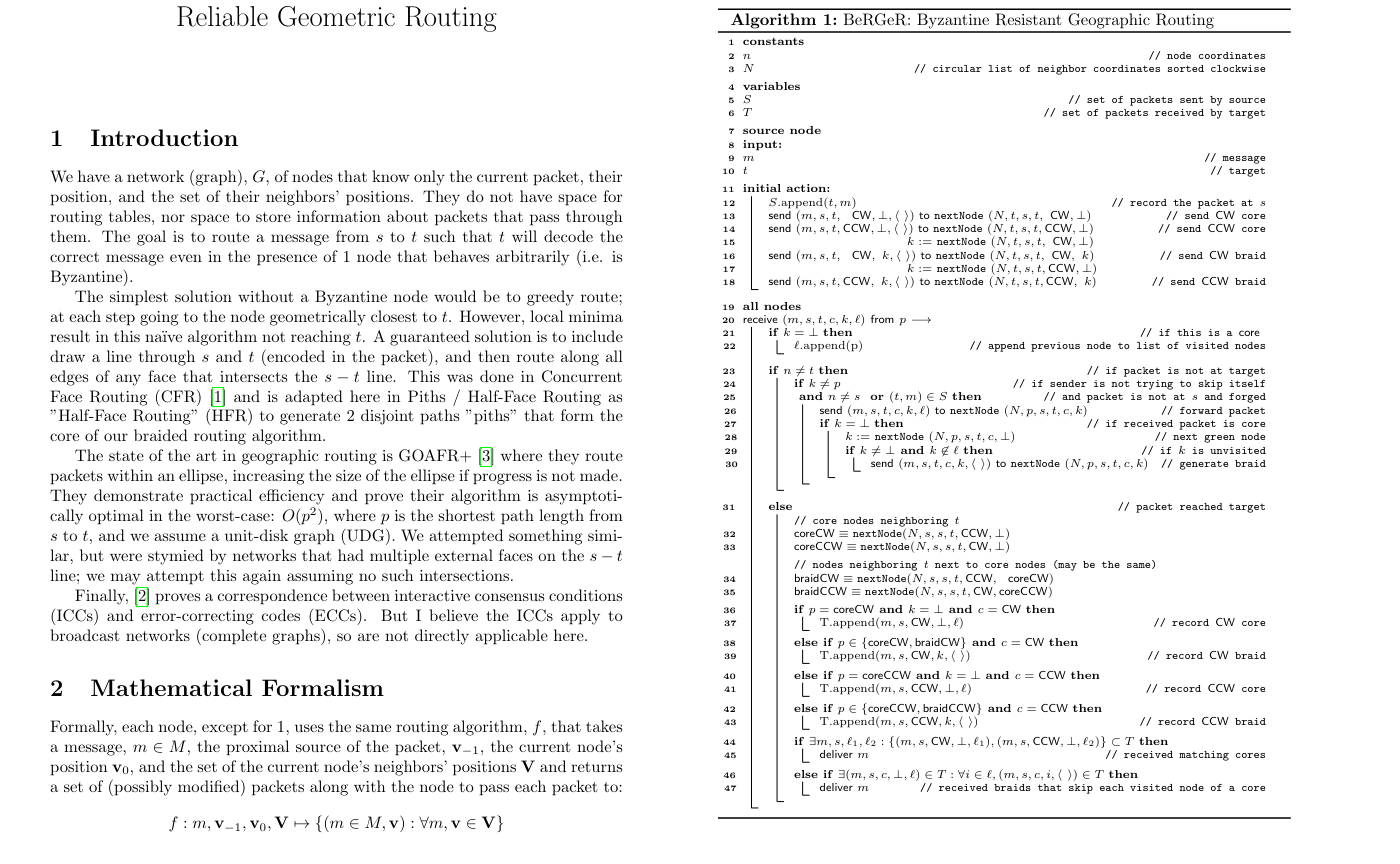
\includegraphics[width=.9\linewidth]{./img/paper.png}
\end{center}
\subsection*{Remove edges that intersect st-line}
\label{sec:org2f8535b}
\begin{center}
\includesvg[width=.9\linewidth]{./img/remove-edges-that-intersect-st}
\end{center}
\subsection*{Proof}
\label{sec:orgbca7f04}
\begin{center}
\includesvg[width=.9\linewidth]{./img/dual-graph}
\end{center}
\subsection*{Proof}
\label{sec:orgab12a8a}
\begin{center}
\includesvg[width=.9\linewidth]{./img/dual-graph-edge-contraction}
\end{center}
\subsection*{Counterexample}
\label{sec:orgb83bca9}
\begin{center}
\includesvg[width=.9\linewidth]{./img/counterexample}
\end{center}
\subsection*{Counterexample}
\label{sec:org952c4eb}
\begin{center}
\includesvg[width=.9\linewidth]{./img/counterexample-faded}
\end{center}
\section*{Acknowledgements}
\label{sec:orgade0fc3}

Prof. Mikhail Nesterenko, for supervising the research

Prof. Gokarna Sharma, for his feedback

Prof. Jenya Soprunova, for her feedback

Prof. Darci Kracht, for advice on the presentation
\section*{Questions?}
\label{sec:org52fd84d}

zaz@zazbrown.com
\end{document}